%===================================== CHAP 5 =================================

\chapter{Result and discussion}
\section{Homogeneous charged block}
\subsection{Homoegeneous charged block outside of nanotube}
In order to investigate the charge property of a polyelectrolyte and the effect of pH and surface halloysite nanotube, we design two fully-charged polyelectrolytes. One is a polyelecrolyte with 40 negatively charged beads and the other is a polyelectrolyte with 40 positively charged beads. The negative polyelectrolyte is for analysing an attractive interaction between positively charged inner surface of alumina and itself, and vice versa.  

First of all, the positive polyelectrolyte adsorbs onto the outer surface at 

    \begin{figure}[h!]
      \centering
        \includegraphics[width=0.5\textwidth]{fig/m40p-snap.jpg}
     \caption{*}
    \label{fig:m40n-snap}
    \end{figure}

    \begin{figure}[h!]
      \centering
        \begin{subfigure}{\linewidth}
          \centering
            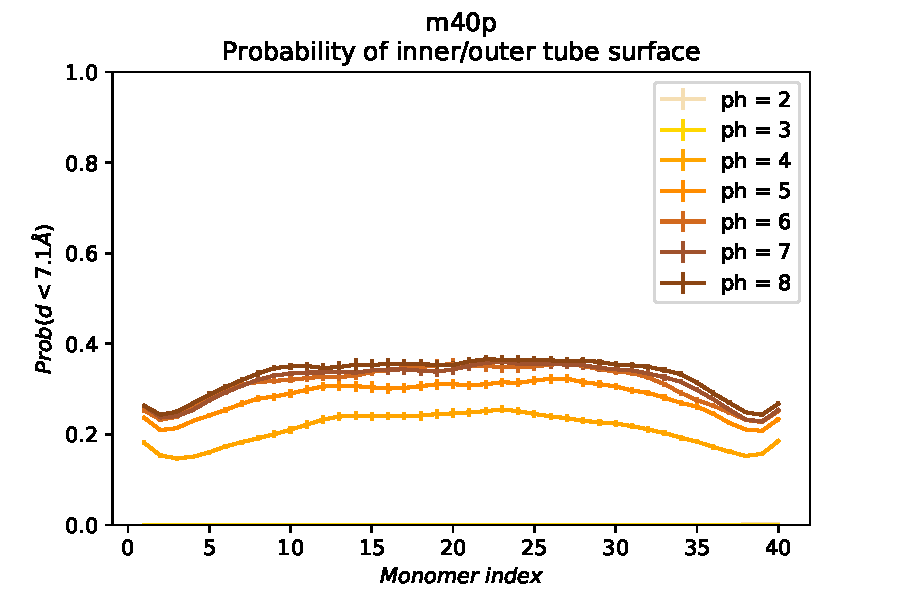
\includegraphics[width=0.5\textwidth]{fig/m40p-prob-io.pdf}  
            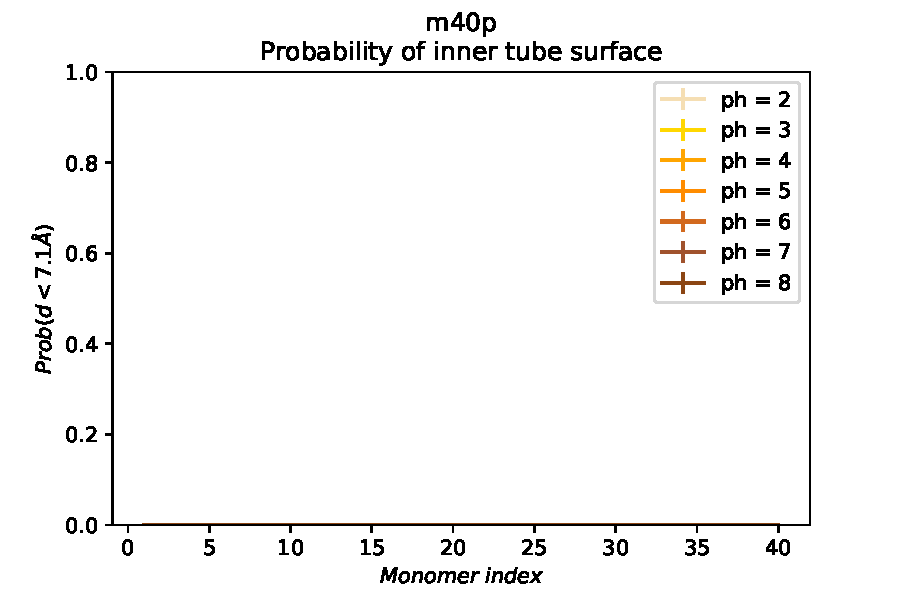
\includegraphics[width=0.5\textwidth]{fig/m40p-prob-i.pdf}
            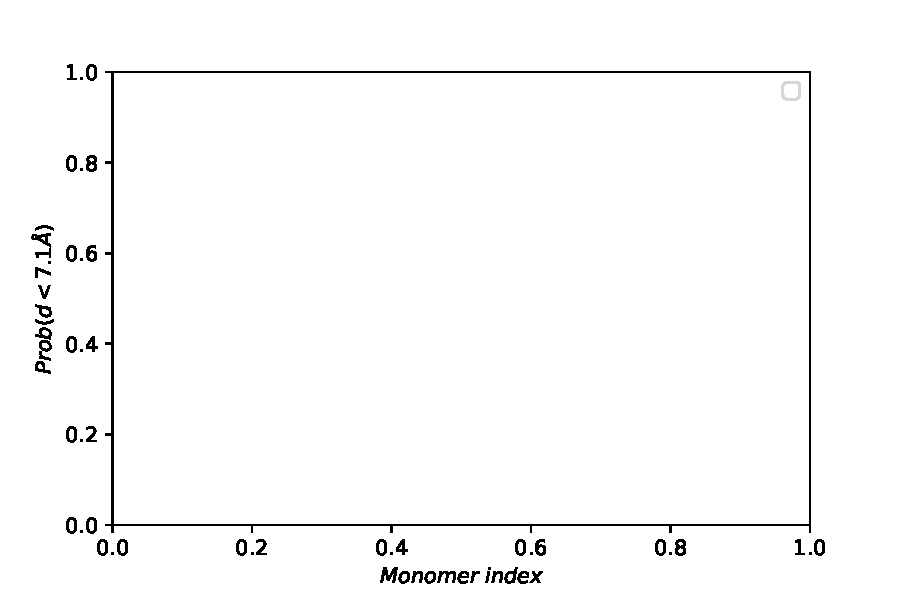
\includegraphics[width=0.5\textwidth]{fig/m40p-prob-o.pdf}
            \end{subfigure}\par\medskip
     \caption{The system with a positively charged polyelectrolyte with 40 monomers and a halloysite nanotube. The probability of adsorbed monomers onto the tube surfaces, (a) the inner surface and outer surface, (b) inner surface only (b) outer surface only. The distance for judging each monomer adsorbs or not is decided with the distance $d = 7.1\AA$. The monomer indices from 0 to 40 is designated to be adsorbed when the center of mass of a monomer bead is located within the range of $d = 7.1\AA$. }
    \label{fig:m40p-prob} %a/b
\end{figure}

\clearpage

We expect the negative polyelectrolyte is attracted to the inner surface and adsorb onto the inner surface of nanotube at pH 2 where the inner surface(Al) is positively charged with the highest fractional ratio of $1.0$ in figure \ref{fig:m40n-frach}, but it doesn't. Even though a repulsive interaction with the outer surface(Si) can be neglected with a very low fractional charge at pH 2 shown in figure \ref{fig:m40n-frach}, the negative polyelectrolyte does not go inside the nanotube as shown in snapshots of figure \ref{fig:m40n-snap}. The negative polyelectrolyte seems like feeling an attractive force with the inner surface but it can not move inside at all. This is also described with the low probability of (a) and (b) in figure ~\ref{fig:m40n-prob} which shows the quantitative degree of how the negative polyelectrolyte adsorbs onto the inner surface. 

\iffalse
    \begin{figure}[h!]
      \centering
        \includegraphics[width=0.5\textwidth]{fig/m40n-snap.jpg}
     \caption{*}
    \label{fig:m40n-snap}
    \end{figure}
\fi

    \begin{figure}[h!]
      \centering
        \begin{subfigure}{\linewidth}
          \centering
            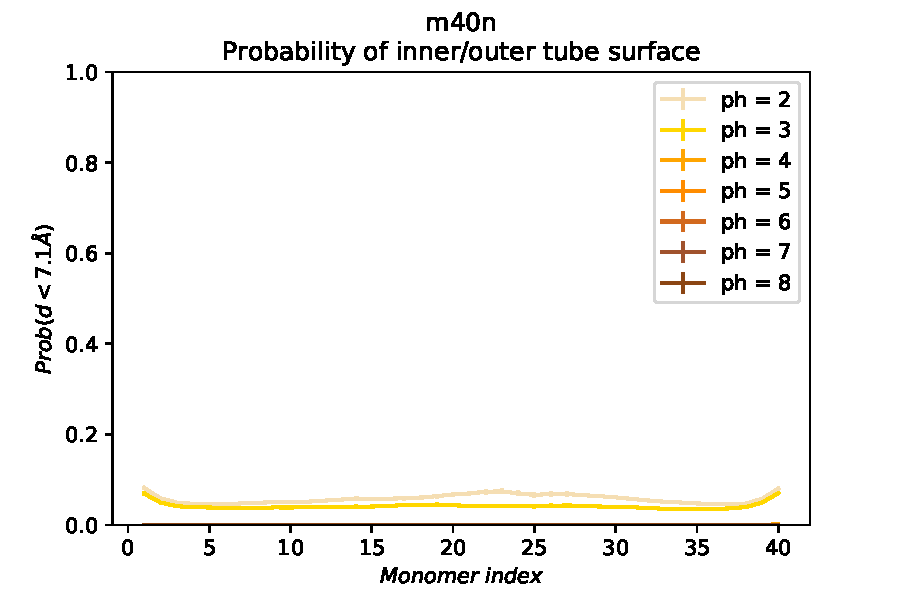
\includegraphics[width=0.5\textwidth]{fig/m40n-prob-io.pdf}  
            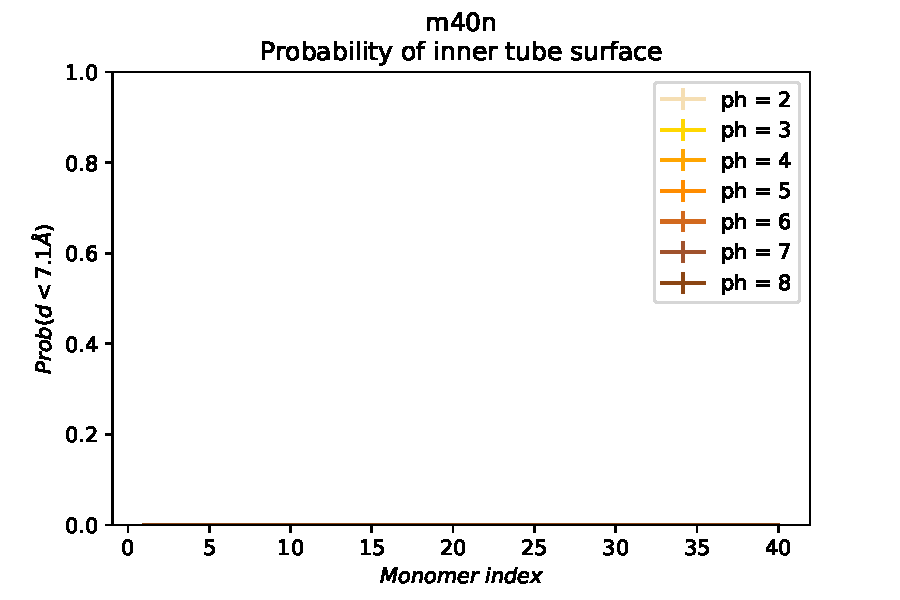
\includegraphics[width=0.5\textwidth]{fig/m40n-prob-i.pdf}
            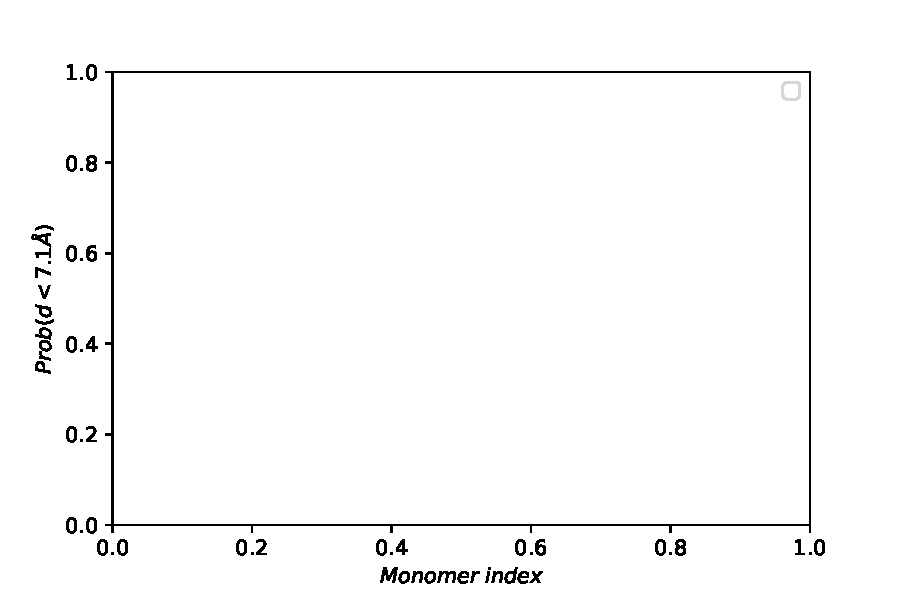
\includegraphics[width=0.5\textwidth]{fig/m40n-prob-o.pdf}
            \end{subfigure}\par\medskip
     \caption{The system with a negatively charged polyelectrolyte with 40 monomers and a halloysite nanotube. The probability of adsorbed monomers onto the tube surfaces, (a) the inner surface and outer surface, (b) inner surface only (b) outer surface only. The distance for judging each monomer adsorbs or not is decided with the distance $d = 7.1\AA$. The monomer indices from 0 to 40 is designated to be adsorbed when the center of mass of a monomer bead is located within the range of $d = 7.1\AA$.  }
    \label{fig:m40n-prob} %a/b
    \end{figure}
    
    \begin{figure}[h!]
      \centering
        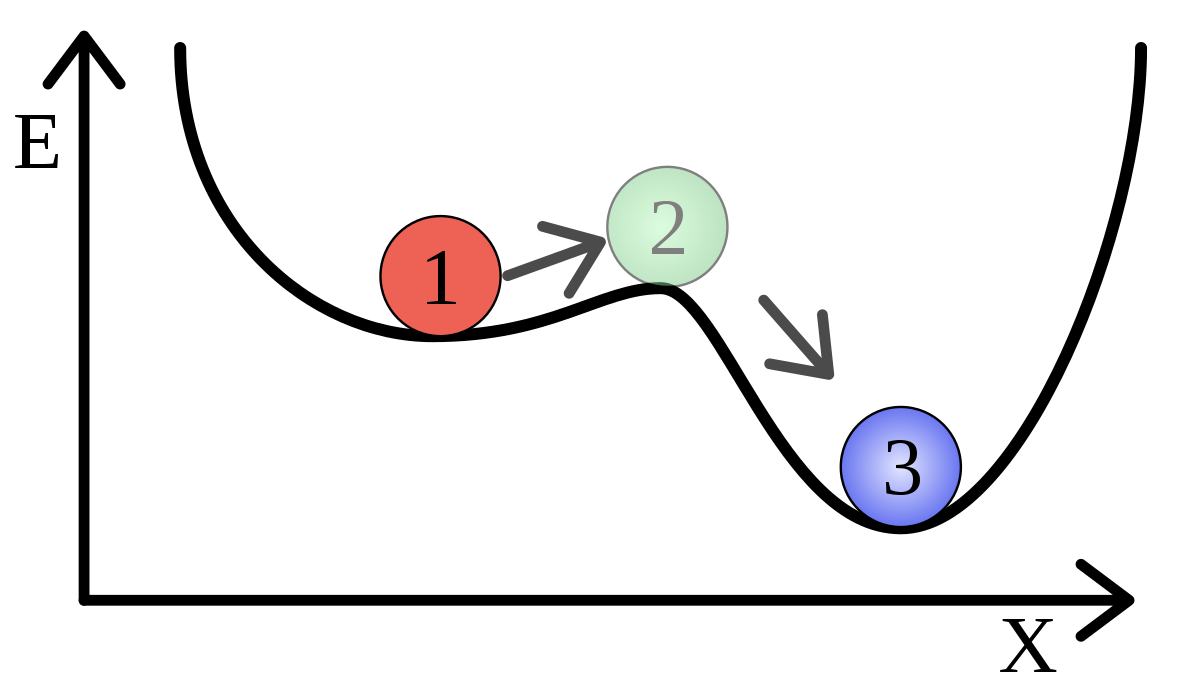
\includegraphics[width=0.5\textwidth]{fig/metastable.png}
     \caption{Fractional charge of the negative polyelectrolyte. Alumina is positively charged at low pH and silica is negatively charged at high pH. }
    \label{fig:m40n-frach}
    \end{figure}

The polyelectrolyte which feels an attractive force but does not come inside the tube can be explained by how this system is modelled. Even though a new configuration of system is acceptable regarding to energy term, an equalibrium state of system can be stuck on one energy well. The movement of monomer beads in the polyelectrolyte is based on random-walk. Therefore, moving many beads into the inner space compensate huge steps and energy than stailizing onto the outer surface in spite of the repulsive interaction between the negative polyelectrolyte and the negative outer silica beads. Shortly, this can be one of the metastable state, not the equalibrium state with the lowest potential energy in this system, as explained in figure \ref{fig:metastable}.\\

    \begin{figure}[h!]
      \centering
        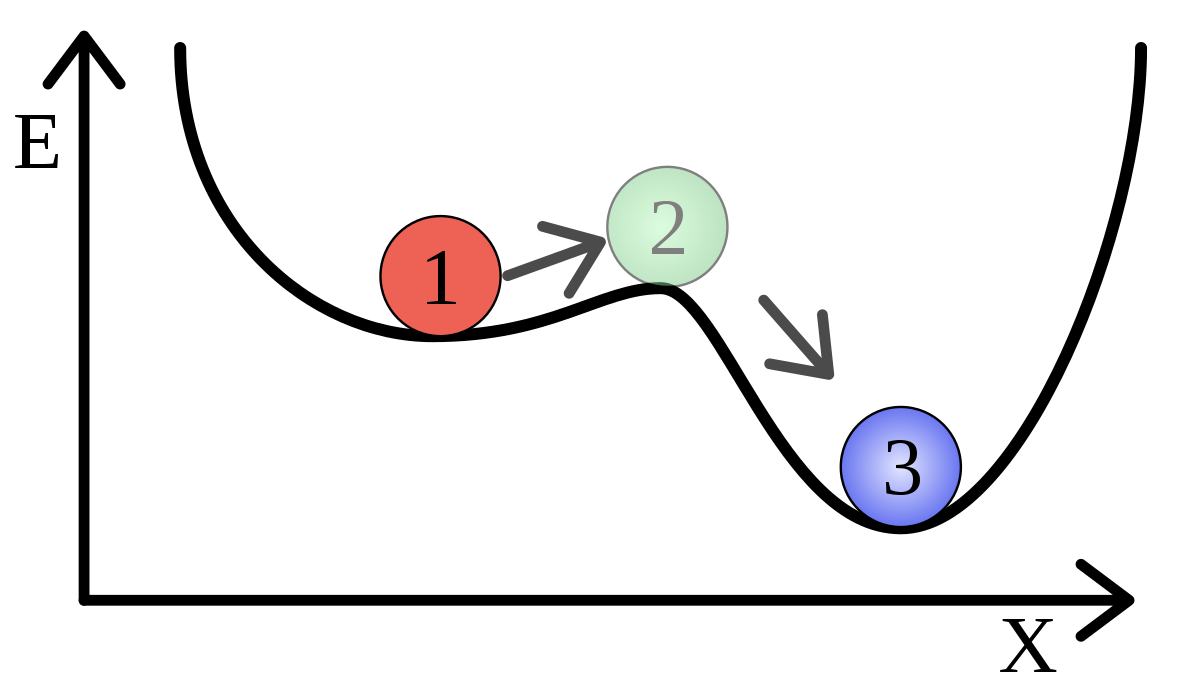
\includegraphics[width=0.5\textwidth]{fig/metastable.png}
     \caption{Explaination of the metastable state. The system is stuck on the metastable state 1 (red) and it needs more energy to move to the lowest state 3 (blue). This process compensate the amount of energy and steps. \ref{*}}
    \label{fig:metastable}
    \end{figure}

For getting this point straight, we execute a same set of simulation with the first configuration of the negative polyelectrolyte starts from a center point of the tube. This is rooted from a hypothesis that the previous results are not basically from the final equalibrium state of the system and the first configuration can affect polymer conformation properties.

%limitation - time - steps 
\clearpage
\subsection{Homogeneous charged block from inside of nanotube}

    \begin{figure}[h!]
      \centering
        \begin{subfigure}{\linewidth}
          \centering
            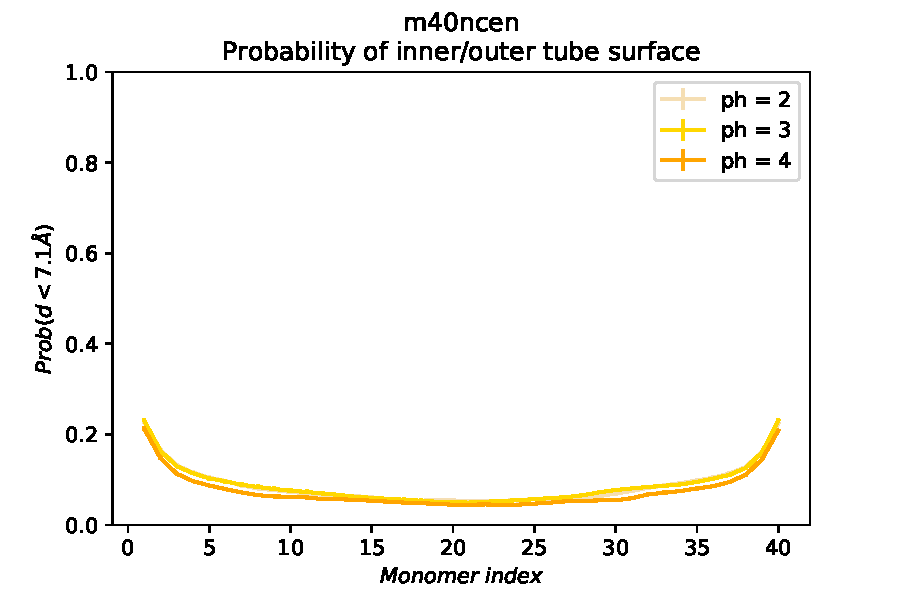
\includegraphics[width=0.5\textwidth]{fig/m40ncen-prob-io.pdf}  
            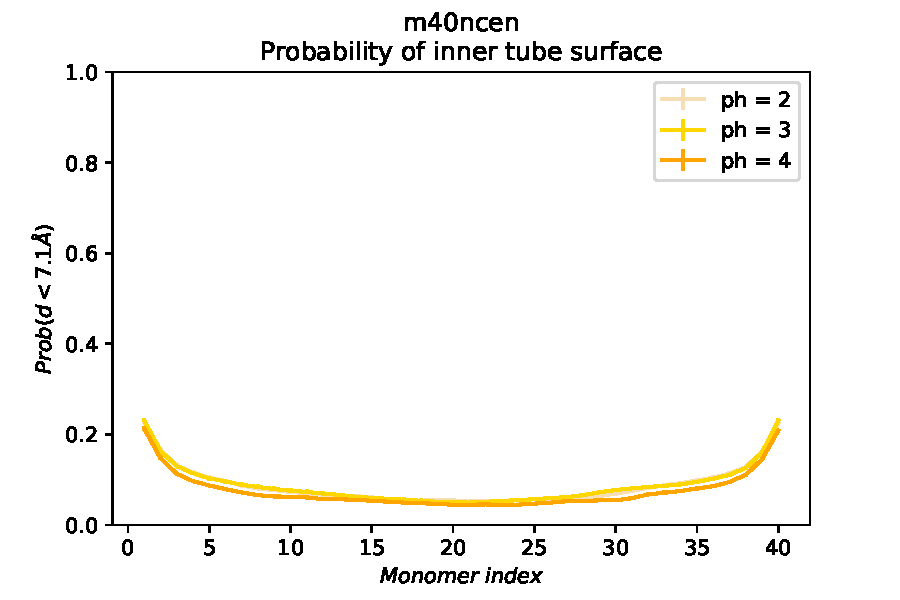
\includegraphics[width=0.5\textwidth]{fig/m40ncen-prob-i.pdf}
            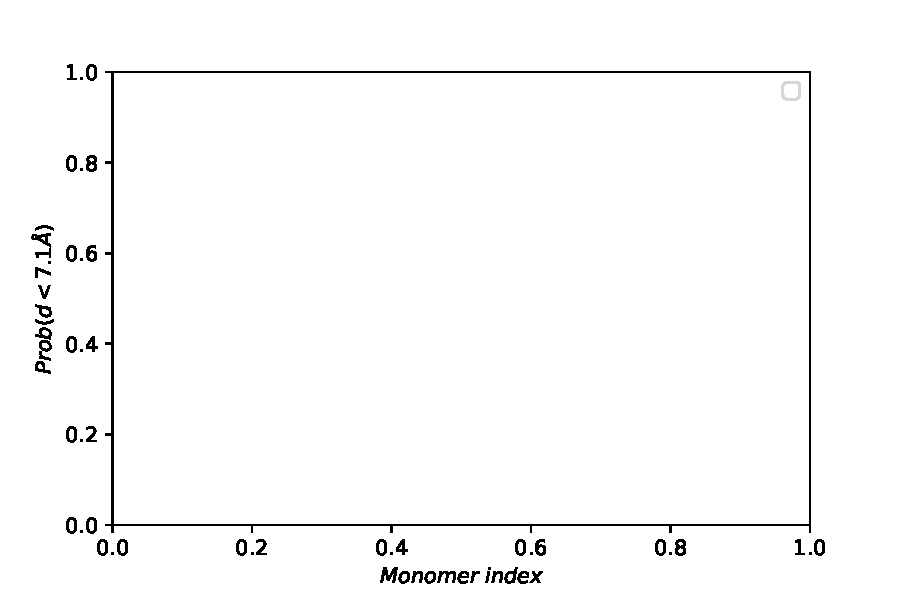
\includegraphics[width=0.5\textwidth]{fig/m40ncen-prob-o.pdf}
            \end{subfigure}\par\medskip
     \caption{The system with a negatively charged polyelectrolyte with 40 monomers and a halloysite nanotube. The polyelectrolyte configuration is made from exactly the center of the (inner) tube. The probability of adsorbed monomers onto the tube surfaces, (a) the inner surface and outer surface, (b) inner surface only (b) outer surface only. The distance for judging each monomer adsorbs or not is decided with the distance $d = 7.1\AA$. The monomer indices from 0 to 40 is designated to be adsorbed when the center of mass of a monomer bead is located within the range of $d = 7.1\AA$.  }
    \label{fig:m40ncen-prob} %a/b
    \end{figure}

    \begin{figure}[h!]
      \centering
        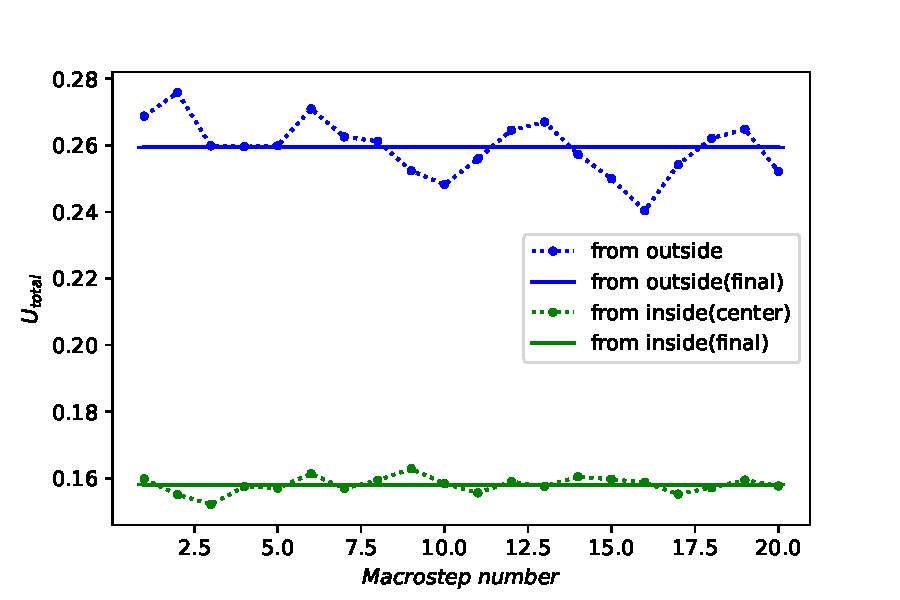
\includegraphics[width=0.5\textwidth]{fig/m40n-m40ncen-u.pdf}
     \caption{Total potential energy of system as increasing macrosteps. The negative polyelectrolyte which starts from inner space of a tube has lower potential energy (Blue line $U_{tot, in, final} = 0.15806$) than the other from outer space of a tube ($U_{tot, out, final} = 0.25935$).}
    \label{fig:m40n-m40ncen-u}
    \end{figure}

    \begin{figure}[h!]
      \centering
        \begin{subfigure}{\linewidth}
          \centering
            \includegraphics[width=0.5\textwidth]{fig/m40pcen-prob-io.pdf}  
            \includegraphics[width=0.5\textwidth]{fig/m40pcen-prob-i.pdf}
            \includegraphics[width=0.5\textwidth]{fig/m40pcen-prob-o.pdf}
            \end{subfigure}\par\medskip
     \caption{The system with a positively charged polyelectrolyte with 40 monomers and a halloysite nanotube. The polyelectrolyte configuration is made from exactly the center of the (inner) tube. The probability of adsorbed monomers onto the tube surfaces, (a) the inner surface and outer surface, (b) inner surface only (b) outer surface only. The distance for judging each monomer adsorbs or not is decided with the distance $d = 7.1\AA$. The monomer indices from 0 to 40 is designated to be adsorbed when the center of mass of a monomer bead is located within the range of $d = 7.1\AA$.  }
    \label{fig:m40ncen-prob} %a/b
    \end{figure}





\noindent
1. potential energy : m40ncen(in) < m40n(out) \\
2. different shape of plot comparing with m40n. \\
- curvature from inside and outside?
3. even thought we make 'easier' circumstance, the probability is not that high. why?

Q. default - where the polymer starts from? anywhere. -0.5*boxlen ~ 0.5*boxlen
 \\



























\cleardoublepage